\chapter{Démarche}
\label{chap:demarche}

Créer des modèles d'architecture d'entreprise à des fins d'analyse par simulation implique de suivre un processus précis. L'objectif de notre travaux est de définir le processus de modélisation et de simulation à adopter, les rôles impliqués, les artefacts conceptuels requis, ainsi que les outils et les langages adéquats pour mener des analyses de structure et de comportement. 

Notre contribution est double. D'abord, nous proposons une démarche de modélisation et d'analyse qui s'appuie sur un cadre d'architecture multi-vues. Nous dotons ce cadre d'architecture d'une vue supplémentaire qui est est la vue intégration. Cette vue a pour but d'adresser les problématiques de cohérence et d'alignement. Ensuite, nous mettons à profit les langages et standards de l'IDM permettant de modéliser et de simuler les architectures d'entreprise. 


%In this section, we present our approach and we apply it on the case study of managing an electric vehicles fleet. Our contribution is twofold. First, we propose a multi-view framework for EA with an additional view: the integration view. This view aims to address consistency and alignment issues. Second, we use executable and standardized languages from MDE to model and simulate EA.


\section{Approche conceptuelle pour la modélisation et l'analyse d'architectures d'entreprise}

L'EA peut avoir différents objectifs. Kurpjuweit et Winter \cite{kurpjuweit2007viewpoint} identifient trois objectifs de l'EA par rapport aux SI de l'entreprise~:~(1)~la documentation et la communication, (2)~l'analyse et la compréhension et (3)~la conception. Nous étendons cette vision centrée sur les SI à l'ensemble de l'entreprise en adoptant l'école de pensée «~intégrative~» comme décrite par la taxonomie de Lapalme (voir section \ref{Lapalme}, page \pageref{Lapalme} de l'état de l'art). 

Nous considérons donc que la documentation et la communication, l'analyse et la compréhension et enfin la conception concernent tout le système entreprise et pas seulement sa composante SI. Par exemple, contrairement à une EA centrée sur les SI, les processus métier sont modélisés et évalués tout autant que l'architecture applicative. La figure \ref{fig:approche_conceptuelle} illustre notre approche conceptuelle. Celle-ci fait intervenir plusieurs types d'acteurs intervenant à plusieurs niveaux de l'entreprise~:
\begin{itemize}
\item un analyste métier qui conçoit la vue métier à travers la modélisation et l'évaluation des processus métier mettant en œuvre la stratégie de l'entreprise~;
\item un architecte fonctionnel qui traduit les processus métier en termes de fonctions logiques~;
\item un architecte applicatif qui traduit la vue fonctionnelle en un ensemble structuré d'applications implémentant les différentes fonctions~;
\item un architecte d'entreprise dont la mission est de mettre en cohérence l'ensemble des vues.
\end{itemize}

\begin{figure}[!htbp]
 \begin{center}
  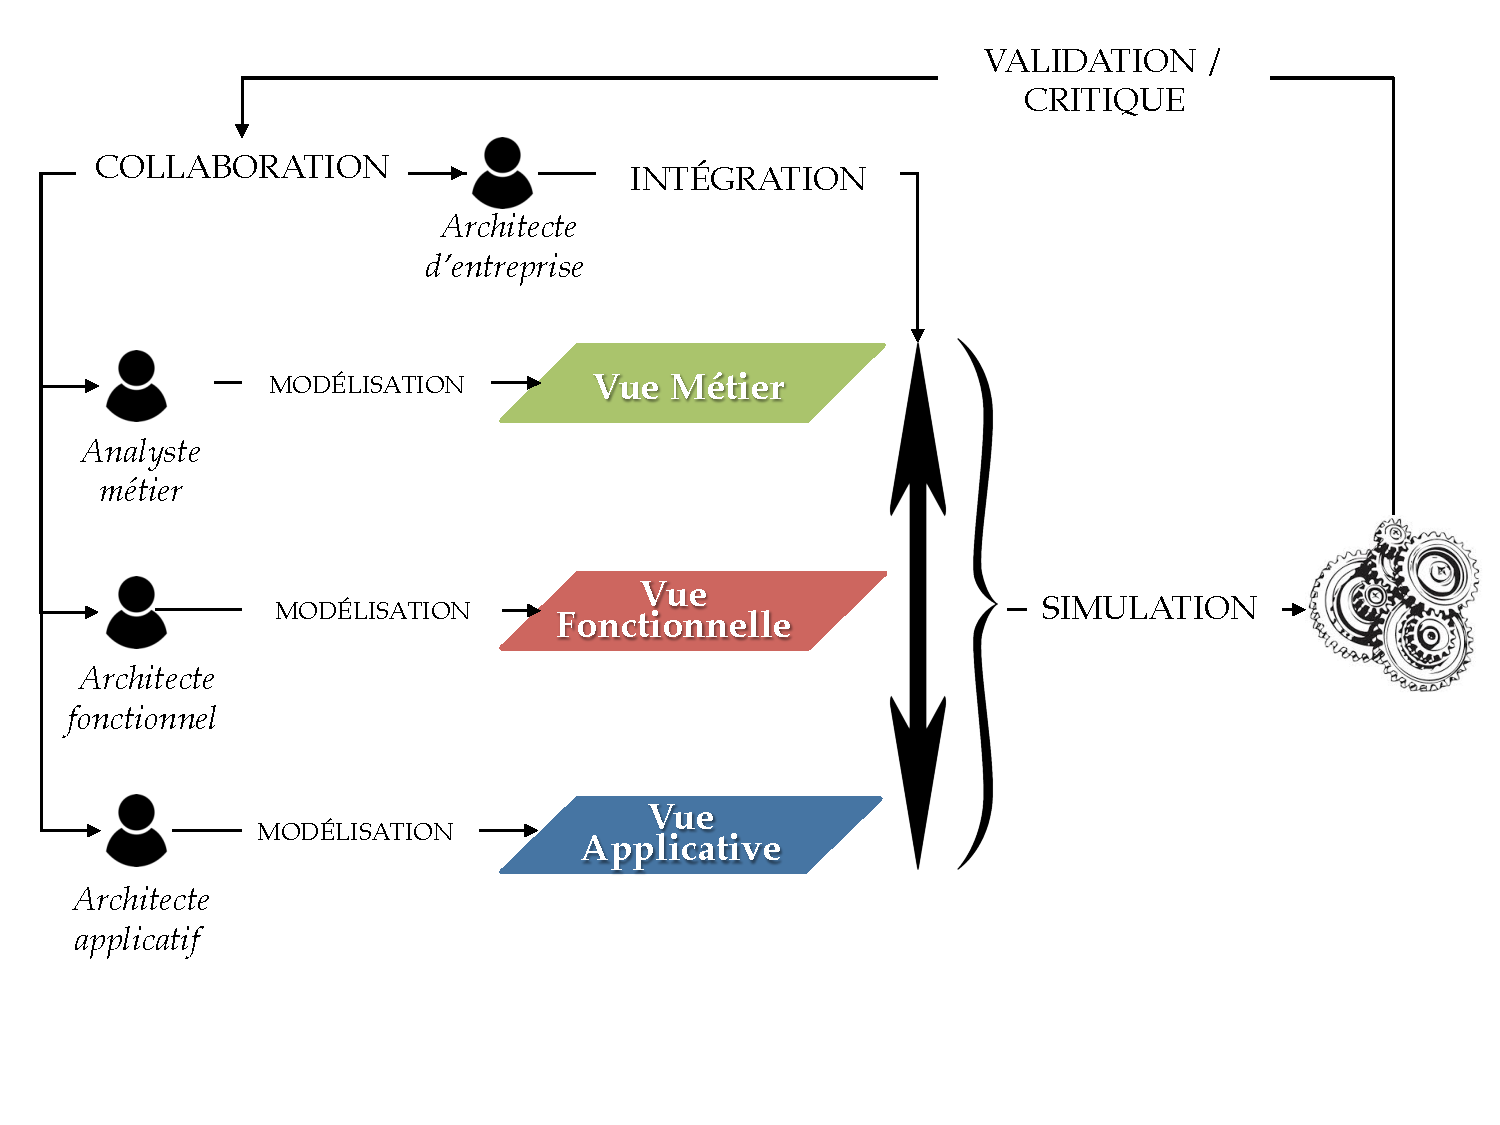
\includegraphics[trim= 0cm 5cm 0cm 0cm, width=1\textwidth]{images/demarche/approche_conceptuelle.pdf}
 \end{center}
 \caption{Approche conceptuelle pour l'analyse d'une architecture d'entreprise}
 \label{fig:approche_conceptuelle}
\end{figure}

L'analyste métier, l'architecte fonctionnel et l'architecte applicatif collaborent entre eux et avec l'architecture d'entreprise pendant tout le processus de modélisation. Par la suite, l'activité d'intégration incombe à l'architecte d'entreprise, détenteur de la vision globale. Mais l'intégration des vues implique de rebouclage avec les autres acteurs (analyste métier, architecte fonctionnel et architecte applicatif) pour garantir l'alignement business/IT. Les étapes de modélisation et d'intégration de notre approche répondent donc aux objectifs de conception et de communication tels que définis par Kurpjuweit et Winter \cite{kurpjuweit2007viewpoint}.

Comme relaté dans l'état de l'art, l'analyse fait partie des activités les moins courantes de l'EA quelle qu'en soit l'école de pensée \cite{chen2008architectures} \cite{barn2013enterprise}. Et même lorsqu'une architecture d'entreprise est analysée très peu d'approches recourent à la simulation pour analyser l'aspect comportemental \cite{glazner2011enterprise} \cite{manzur2015xarchimate}. La simulation est pourtant une technique reconnue pour évaluer le comportement d'un système et/ou évaluer plusieurs stratégies concernant son fonctionnement \cite{shannon1975systems}. Notre approche préconise de simuler les modèles issus de activités de modélisation et d'intégration afin de les valider ou les critiquer par l'ensemble des acteurs impliqués dans l'EA. Nous couvrons ainsi l'objectif d'analyse tel que préconisé par Kurpjuweit et Winter \cite{kurpjuweit2007viewpoint}. 



\section{Un cadre d'architecture dirigé par les modèles exécutables}

Toute simulation d'un système commence par sa modélisation. Pour modéliser des systèmes complexes comme les architectures d'entreprise, nous adoptons une approche par points de vue. Celle-ci facilite la conception des modèles par les acteurs impliqués en séparant leurs préoccupations respectives. Elle permet également de présenter les modèles obtenus, ainsi que les résultats de simulation de manière plus compréhensible à ces acteurs, car chaque point de vue n'utilise que les concepts métier propres à chaque acteur, selon sa perspective. 

Dans notre approche, nous nous intéressons aux vues métier, fonctionnelle et applicative comme l'illustre la figure~\ref{fig:vue_aspect}. Mais nous souhaitons aussi étendre nos travaux à la vue technique. 
Plusieurs raisons motivent l'utilisation de ces points de vue. D'abord, la vue métier et la vue applicative sont incontournables pour n'importe quel cadre d'architecture. Ensuite, selon les cadres d'architecture, la vue fonctionnelle est modélisée de deux manière~:~ elle est soit intégrée à la vue applicative sous forme de services (Archimate, TOGAF, RM-ODP), soit modélisée à part entière dans une vue dédiée (Club Urba, SGAM, Zachman). Nous prenons le parti de modéliser explicitement les fonctions dans une vue dédiée. En effet, passer directement de la vue du métier à la vue applicative peut être en quelque sorte brutal pour l'analyste métier mais aussi pour l'architecte applicatif. La vue fonctionnelle permet une transition progressive de la logique métier vers l'architecture logicielle.

Nous ne modélisons pas les informations dans une vue dédiée contrairement aux cadre RM-ODP ou SGAM. Nous explicitons les informations en tant qu'aspect pour chacune des autres vues comme recommandé par le cadre Zachman (Le quoi de la dimension horizontale). L'aspect «~\textit{information}~» permet d'avoir un modèle explicite des données utilisées dans chacune des vues métier, fonctionnelle et applicative :
	\begin{itemize}
	\item \textbf{L'aspect information du point de vue métier}
	
	Cet aspect établit le modèle de données métier qui  décrit les objets ou concepts métier manipulés par le processus métier. Ce modèle est peu sujet au changement, sauf évolution importante des pratiques métier. Il est aussi à l'origine du découpage en bloc par entité métier de la vue fonctionnelle~;
	\item \textbf{L'aspect information du point de vue fonctionnel}
	
	Cet aspect établit le modèle de données fonctionnelles qui donne le type des données utilisées par les blocs fonctionnels nécessaires à la réalisation de processus métier. Elle décrit leurs caractéristiques et leurs relations sous forme de diagrammes de classes par exemple~;
	
	\item \textbf{L'aspect information du point de vue applicatif} 
	
	Cet aspect établit le modèle de données applicatives qui dépend fortement des applications choisies : il décrit les formats de données compatibles avec les modules applicatifs.
	\end{itemize}
	
\begin{figure}[!htbp]
 \begin{center}
  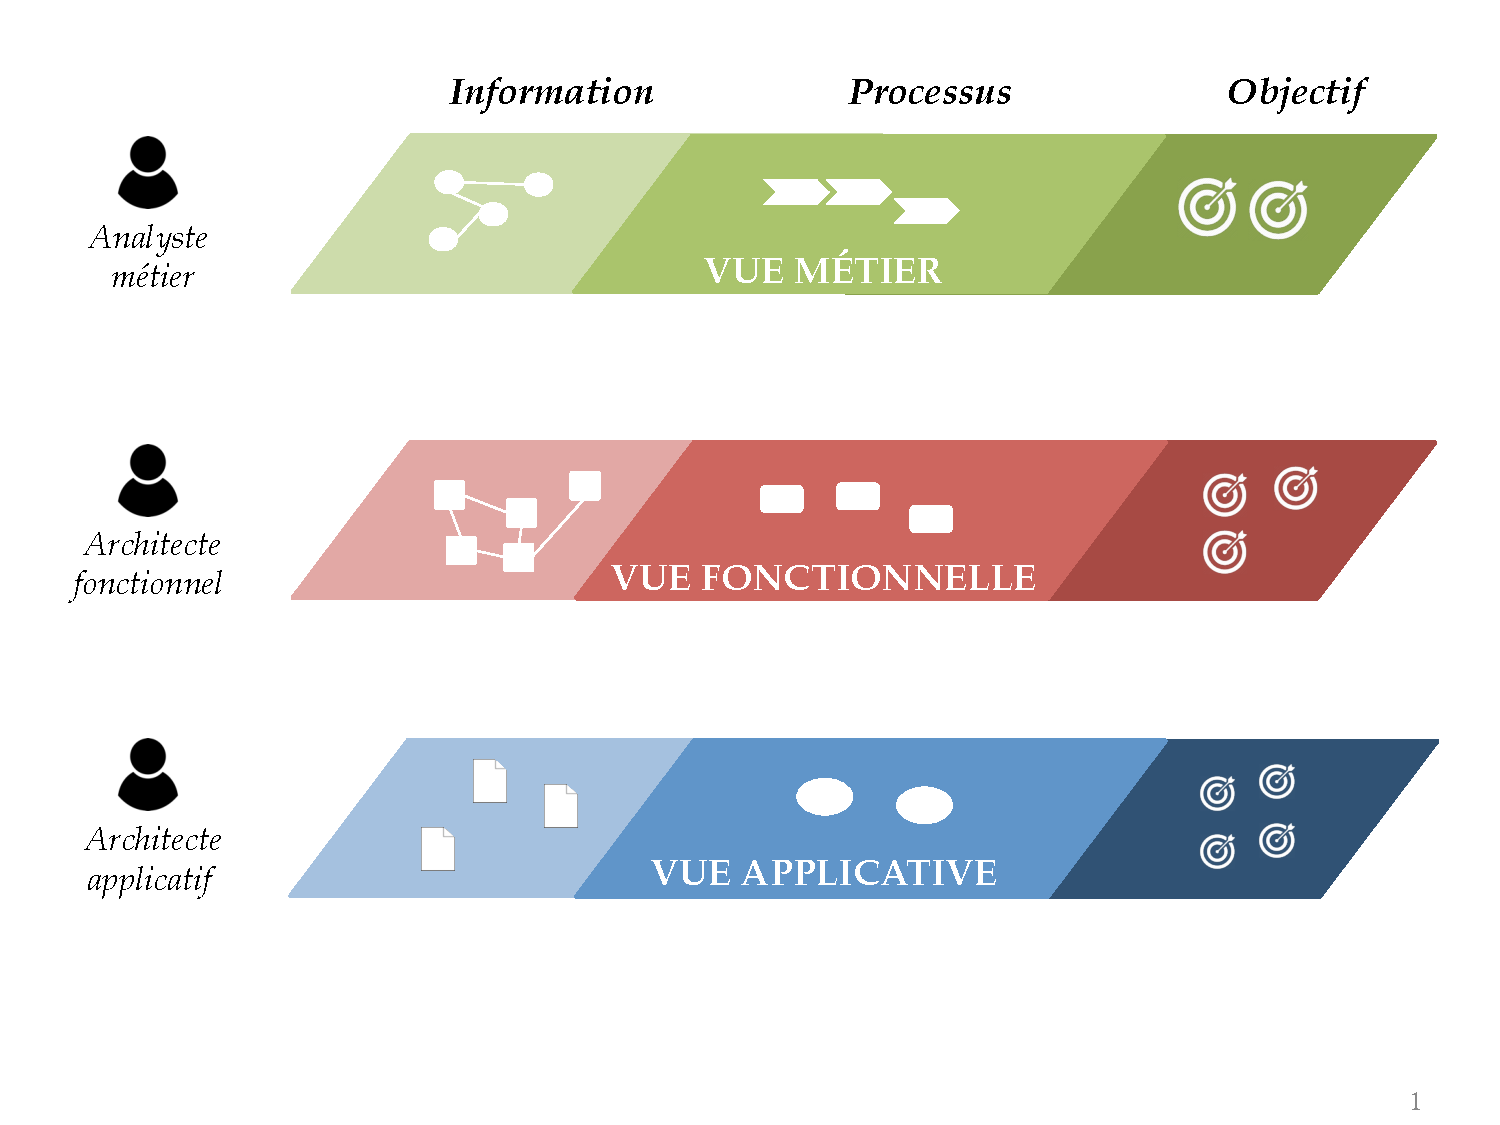
\includegraphics[trim= 0cm 3cm 0cm 0cm, width=1\textwidth]{images/demarche/vue_aspect.pdf}
 \end{center}
 \caption{Points de vue et aspects utilisés}
 \label{fig:vue_aspect}
\end{figure}
	
De plus, nous modélisons le comportement de chaque vue dans l'aspect «~\textit{processus}~». Ainsi nous retrouvons~:

	\begin{itemize}
	\item \textbf{L'aspect processus du point de vue métier} 
	
	Cet aspect correspond aux processus métier de l'entreprise, décrits en utilisant les concepts métier, sans référence aux détails d'implémentation. Nous préconisons l'utilisation de formalismes standard pour la modélisation de processus métier qui soient exécutables, tels que les diagrammes d'activité fUML ou les diagrammes BPMN dans une perspective de simulation. Des langages spécifiques à un domaine (DSML) peuvent également être utilisés~;
	\item \textbf{L'aspect processus d'un point de vue fonctionnel} 
	
	Cet aspect décrit les fonctions qui réalisent les processus métier ainsi que leur orchestration en tant que processus fonctionnels. Ces fonctions sont regroupées en blocs. Chaque objet métier identifié dans l'aspect Information de la vue métier correspond à un unique bloc fonctionnel. Ceci garantit la construction de blocs fonctionnels fortement décorrélés, avec une forte cohésion interne. Dans chaque bloc fonctionnel, on retrouve les opérations correspondant à une tâche donnée du processus qui impacte l'objet métier impliqué~;
	\item \textbf{L'aspect processus du point de vue applicatif}
	
	Cet aspect décrit les modules logiciels qui implantent les blocs fonctionnels ainsi que leur orchestration en processus applicatifs. Dans un premier temps, il est conseillé de dresser un inventaire de l'existant applicatif et d'en extraire les modules capables de réaliser les opérations des blocs fonctionnels. Ensuite, si aucune application ou module existant ne peut répondre au besoin des nouveaux processus métier, l'architecte technique fait le choix des nouveaux composants applicatifs à mettre en place. En plus d'identifier les composants applicatifs existants ou à développer, l'architecte applicatif spécifie leurs interconnexions tels que échange de messages, synchronisation de données, transfert de fichiers périodique.
	\end{itemize}
	
Nous étendons chacune des vues par l'aspect «~\textit{objectif}~». Cet aspect correspond au «~\textit{pourqoi}~» du cadre Zachman qui spécifie les motivations de l'architecture. D'une part, modéliser cet aspect permet de garder une traçabilité d'une entre les processus modélisés et les objectifs qu'ils sont censés remplir. D'autre part, il permet de décliner les objectifs métier en objectifs applicatifs, et les objectifs applicatifs en objectifs fonctionnels. Comme nos travaux adoptent l'école de pensée «~Architecture du Système Entreprise~», nous souhaitons évaluer non seulement la composante SI mais l'ensemble de l'entreprise dont la stratégie. L'aspect objectif est un moyen de modéliser explicitement la stratégie de l'entreprise, traduite en un ensemble cohérent d'objectifs métier, en vue (1) d'évaluer la capacité des processus mis en place à y répondre et (2) d'évaluer la stratégie elle-même par rapport à la réalité de l'entreprise. 
 
\begin{figure}[!htbp]
 \begin{center}
  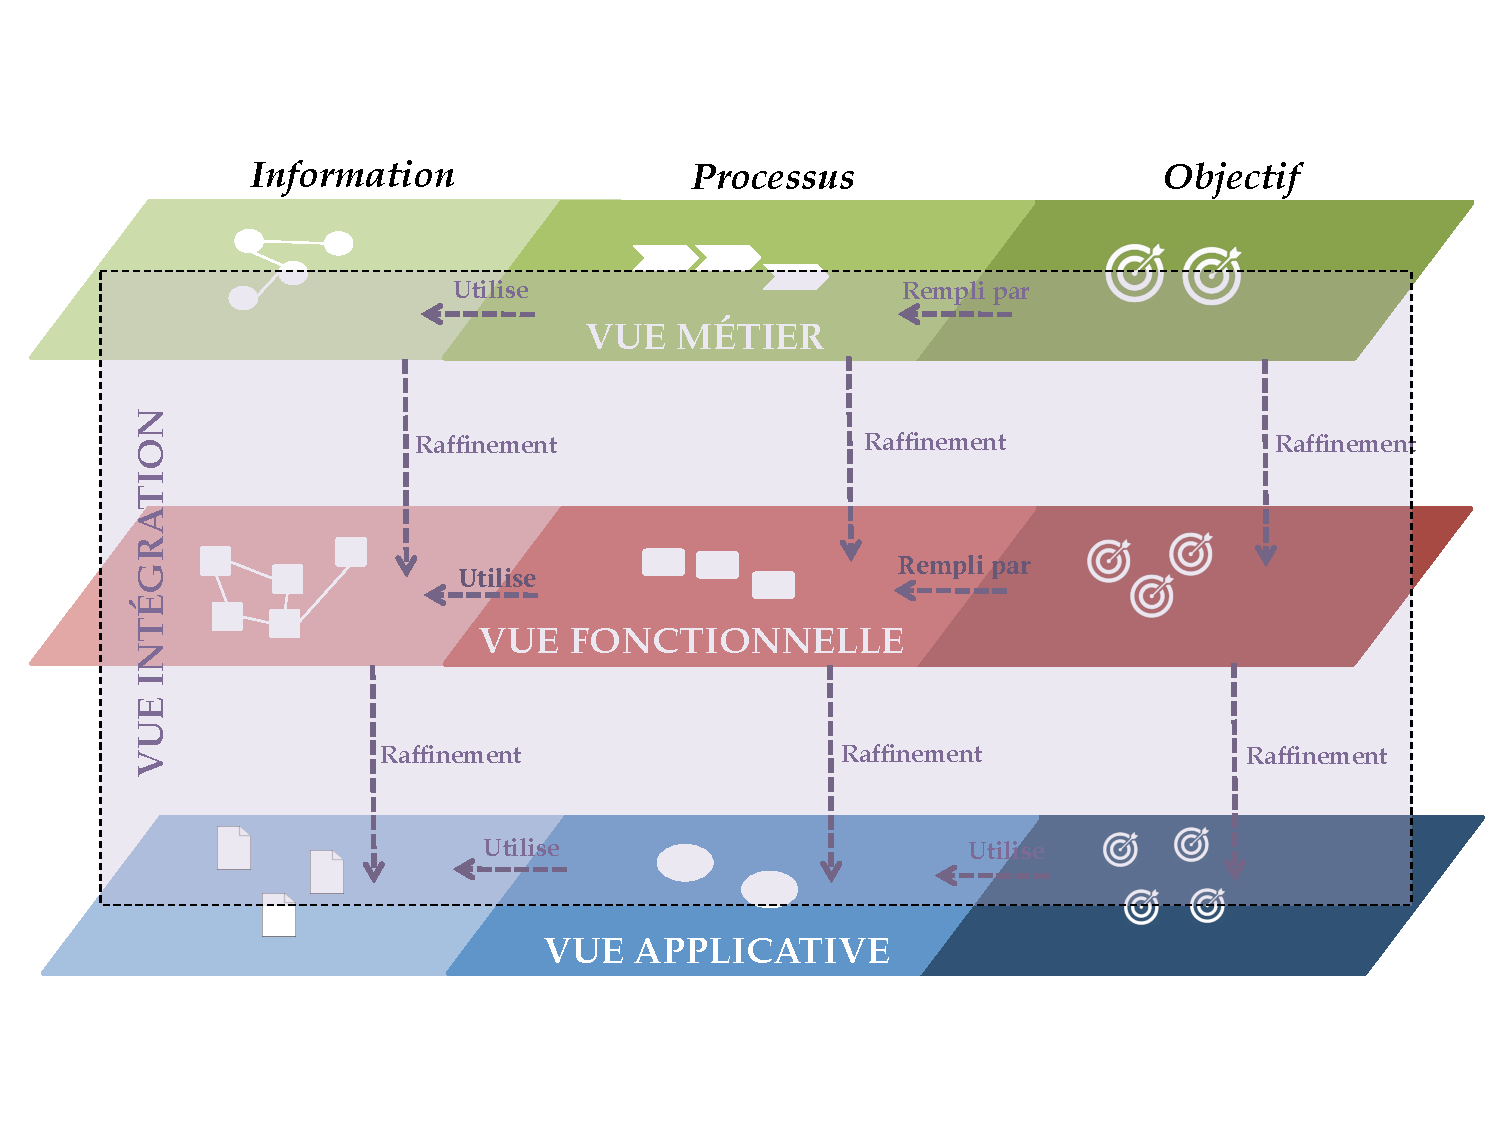
\includegraphics[trim= 3cm 3cm 0cm 0cm, width=1\textwidth]{images/demarche/vue_integration.pdf}
 \end{center}
 \caption{Vue Intégration}
 \label{fig:vue_integration}
\end{figure}

It is a requirement that the enterprise concepts and
models should be simple enough so that they may be used as a communication, analysis and discussion
tool.

The enterprise models need to be defined with simple common sense rules, but also
be sound and coherent. This means the models must provide a high-level view that abstracts
technical details and interconnections while keeping a complex structure traceable and coherent. 

 

%(Describes the system’s functional elements, their responsibilities, interfaces, and primary interactions. A Functional view is the cornerstone of most ADs and is often the first part of the description that stakeholders try to read. It drives the shape of other system structures such as the information structure, concurrency structure, deployment structure, and so on. It also has a significant impact on the system’s quality properties such as its ability to change, its ability to be secured, and its runtime performance.)






